\documentclass{beamer}


\def\A {\ensuremath{\mathbb{A}}}
\def\B {\ensuremath{\mathbb{B}}}
\def\C {\ensuremath{\mathbb{C}}}
\def\D {\ensuremath{\mathbb{D}}}
\def\F {\ensuremath{\mathbb{F}}}
\def\K {\ensuremath{\mathbb{K}}}
\def\L {\ensuremath{\mathbb{L}}}
\def\M {\ensuremath{\mathsf{M}}}
\def\N {\ensuremath{\mathbb{N}}}
\def\Q {\ensuremath{\mathbb{Q}}}
\def\R {\ensuremath{\mathbb{R}}}
\def\T {\ensuremath{\mathcal{T}}}
\def\Z {\ensuremath{\mathbb{Z}}}
%% \def\Z {\ensuremath{{Z}}}
\newcommand{\qub}{\overline{\mathbb{Q}}}

\newcommand{\Le}{\leqslant}
\newcommand{\Ge}{\geqslant}

%% \DeclareMathOperator{\rank}{rank}
\DeclareMathOperator{\Char}{char}
\DeclareMathOperator{\Rem}{\sf d-rem}
\DeclareMathOperator{\drem}{\sf d-rem}
\DeclareMathOperator{\ord}{ord}
\DeclareMathOperator{\charact}{char}
\DeclareMathOperator{\Quot}{Quot}




\definecolor{greyB}{rgb}{0.1,0.1,0.35}
\definecolor{grey}{rgb}{0.5,0.5,0.5}
\definecolor{red1}{rgb}{1,0,0}
\definecolor{blue1}{rgb}{0,0,1}
\definecolor{grey1}{rgb}{0.7,0.7,0.7}

\definecolor{darkred}{rgb}{0.5,0,0}
\definecolor{darkblue}{rgb}{0,0,0.5}
\definecolor{darkgreen}{rgb}{0,0.6,0}
\definecolor{lightred}{rgb}{1,0.5,0.5}
\definecolor{lightblue}{rgb}{0.7,0.7,1}
\definecolor{magenta1}{cmyk}{0.1,0.8,0.3,0.1}
\definecolor{magenta2}{cmyk}{0.1,0.8,1,0.1}
\definecolor{magenta3}{cmyk}{0.2,0.9,1,0.1}
\definecolor{magenta4}{cmyk}{0.3,0.7,1,0.1}
\definecolor{cdef}{rgb}{0,0,0.5}
\definecolor{cdef2}{rgb}{0.6,0.6,1}
\definecolor{DarkGreen1}{rgb}{0.6000,1,0.600}
\definecolor{cdef3}{rgb}{0.5,0,0.3}
\definecolor{cemph}{rgb}{0,0.5,0}
\definecolor{mycolor}{rgb}{0.9,0.04,0.02}
\definecolor{mycolor1}{rgb}{0.9,0.54,0.52}
\definecolor{mydarkblue}{rgb}{0,0.08,0.45}
\definecolor{col0}{rgb}{0.000,0.000,0.000}
\definecolor{col1}{rgb}{0.000,0.000,1.000}
\definecolor{col2}{rgb}{0.000,1.000,0.000}
\definecolor{col3}{rgb}{0.000,1.000,1.000}
\definecolor{col4}{rgb}{1.000,0.000,0.000}
\definecolor{col5}{rgb}{1.000,0.000,1.000}
\definecolor{Yellow}{rgb}{1.000,1.000,0.000}
\definecolor{col7}{rgb}{1.000,1.000,1.000}
\definecolor{Darkblue}{rgb}{0.000,0.000,0.560}
\definecolor{Blue}{rgb}{0.000,0.000,0.690}
\definecolor{Lightblue}{rgb}{0.000,0.000,0.820}
\definecolor{VeryLightBlue}{rgb}{0.530,0.810,1.000}
\definecolor{DarkGreen}{rgb}{0.000,0.360,0.000}
\definecolor{Green}{rgb}{0.000,0.690,0.000}
\definecolor{LightGreen}{rgb}{0.000,0.820,0.000}
\definecolor{Aquamarine}{rgb}{0.000,0.690,0.690}
\definecolor{col17}{rgb}{0.000,0.820,0.820}
\definecolor{RedViolet}{rgb}{0.560,0.000,0.000}
\definecolor{RubineRed}{rgb}{0.690,0.000,0.000}
\definecolor{WildStrawberry}{rgb}{0.820,0.000,0.000}
\definecolor{Violet}{rgb}{0.560,0.000,0.560}
\definecolor{col22}{rgb}{0.690,0.000,0.690}
\definecolor{col23}{rgb}{0.820,0.000,0.820}
\definecolor{Brown}{rgb}{0.500,0.190,0.000}
\definecolor{col25}{rgb}{0.630,0.250,0.000}
\definecolor{Bitter}{rgb}{0.750,0.380,0.000}
\definecolor{Pink}{rgb}{1.000,0.500,0.500}
\definecolor{col28}{rgb}{1.000,0.630,0.630}
\definecolor{col30}{rgb}{1.000,0.880,0.880}
\definecolor{Dandelion}{rgb}{1.000,0.840,0.000}
\definecolor{Turquoise}{rgb}{1.00,0.860,0.860}


\newcommand{\heading}[1]{
  \begin{center}
   {\large\bf{{\textcolor{Blue}{#1}}}}
  \end{center}
  \vspace{1ex}
}
\newcommand{\sheading}[1]{
  \begin{center}
   {\large\bf{\em{{\textcolor{RedViolet}{#1}}}}}
  \end{center}
  \vspace{1ex}
}

\newcommand{\Mblue}[1]{\mbox{\textcolor{blue}{$#1$}}}
\newcommand{\Mcyan}[1]{\mbox{\textcolor{cyan}{$#1$}}}
\newcommand{\Mmagenta}[1]{\mbox{\textcolor{magenta}{$#1$}}}
\newcommand{\Mgreen}[1]{\mbox{\textcolor{green}{$#1$}}}
\newcommand{\Myellow}[1]{\mbox{\textcolor{yellow}{$#1$}}}
\newcommand{\Mtomato}[1]{\mbox{\textcolor{red}{$#1$}}}

\newcommand{\red}[1]{\mbox{\textcolor{red}{#1}}}
\newcommand{\blue}[1]{\mbox{\textcolor{blue}{#1}}}

\newcommand{\colordef}[1]{\mbox{\bf{{\textcolor{red1}{#1}}}}}
\newcommand{\colorem}[1]{\mbox{ \bf{{\textcolor{darkgreen}{#1}}}}}
\newcommand{\colorEM}[1]{\mbox{ \bf{{\textcolor{magenta1}{#1}}}}}
\newcommand{\colorenv}[1]{\mbox{ \bf{{\textcolor{Brown}{#1}}}}}

%%%%%%%%%%%%%%%%%%%%%%%%%%%%%%%%%%%%%%%%%%%%%%
%       For Triangular Decomposition
%%%%%%%%%%%%%%%%%%%%%%%%%%%%%%%%%%%%%%%%%%%%%%
\newcommand{\degree}[1]{\mbox{{\rm degree}$(#1)$}}
\newcommand{\init}[1]{\mbox{{\rm init}$(#1)$}}
\newcommand{\iter}[1]{\mbox{{\rm iter}$(#1)$}}
\newcommand{\mdeg}[1]{\mbox{{\rm mdeg}$(#1)$}}
\newcommand{\mvar}[1]{\mbox{{\rm mvar}$(#1)$}}
\newcommand{\prem}[1]{\mbox{{\rm prem}$(#1)$}}
\newcommand{\pquo}[1]{\mbox{{\rm pquo}$(#1)$}}
\newcommand{\rank}[1]{\mbox{{\rm rank}$(#1)$}}
\newcommand{\res}[1]{\mbox{{\rm res}$(#1)$}}
\newcommand{\sat}[1]{\mbox{{\rm sat}$(#1)$}}
\newcommand{\sep}[1]{\mbox{{\rm sep}$(#1)$}}
\newcommand{\tail}[1]{\mbox{{\rm tail}$(#1)$}}
\newcommand{\disc}[1]{\mbox{{\rm disc}$(#1)$}}
\newcommand{\alg}[1]{\mbox{{\rm alg}$(#1)$}}
\newcommand{\collectUpper}[2]{\mbox{ ${#1}_{#2}^{+}$}}
\newcommand{\collectUnder}[2]{\mbox{ ${#1}_{#2}^{-}$}}
\newcommand{\select}[2]{\mbox{ ${#1}_{#2}$}}
\newcommand{\trdred}[1]{\mbox{{\sf red}$(#1)$}}
\newcommand{\dimension}[1]{\mbox{{\sf dim}$(#1)$}}
\newcommand{\pseudoremainder}[1]{\mbox{{\rm prem}$(#1)$}}
\newcommand{\pseudoquotient}[1]{\mbox{{\rm pquo}$(#1)$}}
\newcommand{\pseudodivision}[1]{\mbox{{\rm pdivide}$(#1)$}}
\newcommand{\euclideanDivision}[4]{\mbox{{$ \begin{array}{c|c} #1 & #2 \\ \cline{2-2}
                                                               #3 & #4 \\ \end{array} $}}}
\newcommand{\multivariateDivisionsix}[6]{\mbox{{$ \begin{array}{c|c|c} #1 & #2 & #3   \\ \cline{2-3}
                                                                     #4 & #5 & #6 \\ \end{array} $}}}
\newcommand{\multivariateDivisionhuit}[8]{\mbox{{$ \begin{array}{c|c|c|c} #1 & #2 & #3 & #4  \\ \cline{2-4}
                                                                       #5 & #6 & #7 & #8 \\ \end{array} $}}}

\newcommand{\conv}{\mathop{\rm conv}\nolimits}
\newcommand{\ld}{\mathop{\rm ld}\nolimits}
\newcommand{\lm}{\mathop{\rm lm}\nolimits}
\newcommand{\lc}{\mathop{\rm lc}\nolimits}
\newcommand{\lp}{\mathop{\rm lp}\nolimits}
\newcommand{\lv}{\mathop{\rm lv}\nolimits}
\newcommand{\NormalForm}[1]{\mbox{{\rm NormalForm}$(#1)$}}

\newcommand{\Init}{\mathop{\mathbb {\rm I}}\nolimits}
\newcommand{\Sep}{\mathop{\mathbb {\rm S}}\nolimits}
\newcommand{\Ld}{\mathop{\rm Ld}}
\newcommand{\Rk}{\mathop{\rm Rk}}
\newcommand{\rk}{\mathop{\rm rk}\nolimits}
\newcommand{\rkchar}{\mathop{\rm rkchar}\nolimits}
\newcommand{\wrk}{\mathop{\rm wrk}\nolimits}
\newcommand{\allrk}{\mathop{\rm allrk}\nolimits}
\newcommand{\algrem}{\mbox{\sf alg-rem}}
\newcommand{\partrem}{\mbox{\sf part-rem}}
\newcommand{\fullrem}{\mbox{\sf full-rem}}
\newcommand{\saturate}[1]{\mbox{{\rm Sat}$(#1)$}}
\newcommand{\leadingCoefficient}[1]{\mbox{{\rm lc}$(#1)$}}
\newcommand{\leadingMonomial}[1]{\mbox{{\rm lm}$(#1)$}}
\newcommand{\leadingTerm}[1]{\mbox{{\rm lt}$(#1)$}}
\newcommand{\setsize}[1]{\mbox{$ | #1 | $}}

\def\jac {\ensuremath{{\mathrm{Jac}}}}
\newcommand{\Autoreduce}{\mathop{\sf Autoreduce}}

\def\pu {\ensuremath{\textcolor{blue}{p_1}}}
\def\pd {\ensuremath{\textcolor{red}{p_2}}}

\def\var{\ensuremath{\mathbf{V}}}
\def\zero{\ensuremath{\mathbf{Z}}}
\def\W{\ensuremath{\mathbf{W}}}
\def\D{\ensuremath{\mathbf{D}}}
\def\KK {\ensuremath{\overline{\mathbb{K}}}}

%%%%%%%%%%%%%%%%%%%%%%%%%%%%%%%%%%%%%%%%%%%%%%
%       For Subresultants
%%%%%%%%%%%%%%%%%%%%%%%%%%%%%%%%%%%%%%%%%%%%%%
\newcommand{\dpol}[1]{\mbox{{\rm dpol}$(#1)$}}
\newcommand{\mat}[1]{\mbox{{\rm mat}$(#1)$}}
%% \newcommand{\det}[1]{\mbox{{\rm det}$(#1)$}}
\newcommand{\fr}[1]{\mbox{{\rm fr}$(#1)$}}
\newcommand{\lsr}[1]{\mbox{{\rm lsr}$(#1)$}}
\newcommand{\src}[1]{\mbox{{\rm src}$(#1)$}}
\newcommand{\resultant}[1]{\mbox{{\sf res}$(#1)$}}

%%%%%%%%%%%%%%%%%%%%%%%%%%%%%%%%%%%%%%%%%%%%%%
% For the RegularChains library (functions)
%%%%%%%%%%%%%%%%%%%%%%%%%%%%%%%%%%%%%%%%%%%%%%
\newcommand{\RegularChainRegularize}{\sc {Regularize}}
\newcommand{\Normalize}[1]{\mbox{{\rm Normalize}$(#1)$}}
\newcommand{\IsUnit}[1]{\mbox{{\rm IsInvertible}$(#1)$}}
\newcommand{\RegularGcd}[1]{\mbox{{\rm RegularGcd}$(#1)$}}
\newcommand{\MainVariable}[1]{\mbox{{\rm MainVariable}$(#1)$}}
\newcommand{\Initial}[1]{\mbox{{\rm Initial}$(#1)$}}
\newcommand{\Intersect}[1]{\mbox{{\rm Intersect}$(#1)$}}
\newcommand{\Extend}[1]{\mbox{{\rm Extend}$(#1)$}}
\newcommand{\GenericSolve}[1]{\mbox{{\rm GenericSolve}$(#1)$}}
\newcommand{\Lift}[1]{\mbox{{\rm Lift}$(#1)$}}

%%%%%%%%%%%%%%%%%%%%%%%%%%%%%%%%%%%%%%%%%%%%%%
%      For FastTriade
%%%%%%%%%%%%%%%%%%%%%%%%%%%%%%%%%%%%%%%%%%%%%%
\newcommand{\IsInvertible}{\sc {IsInvertible}}
\def\FFT{\ensuremath{\mathrm{FFT}}}
\def\TFT{\ensuremath{\mathrm{TFT}}}
\def\DFT{\ensuremath{\mathrm{DFT}}}

%%%%%%%%%%%%%%%%%%%%%%%%%%%%%%%%%%%%%%%%%%%%%%
%     For Software
%%%%%%%%%%%%%%%%%%%%%%%%%%%%%%%%%%%%%%%%%%%%%%
\newcommand{\AXIOM}{{\sc AXIOM}}
\newcommand{\axiom}{{\sc axiom}}
\newcommand{\Aldor}{{\sc Aldor}}
\newcommand{\aldor}{{\sc Aldor}}
\newcommand{\maple}{{\sc Maple}}
\newcommand{\Maple}{{\sc Maple}}
\newcommand{\Triade}{{\sf Triade}}
\newcommand{\FastTriade}{{\sf FastTriade}}
\newcommand{\BasicMath}{{\sf BasicMath}}
\newcommand{\RegularChains}{{\tt RegularChains}}
\newcommand{\lisp}{{\sc Lisp}}
\newcommand{\spad}{{\sc SPAD}}
\newcommand{\gnu}{\mbox{{\sc GNU}}}
\newcommand{\gmp}{\mbox{{\sc GMP}}}
\newcommand{\gcl}{\mbox{{\sc GCL}}}
\newcommand{\ntl}{\mbox{{\sc NTL}}}
\newcommand{\assembly}{\mbox{{\sc Assembly}}}
\newcommand{\cc}{\mbox{{\sc C}}}
\newcommand{\Epsilon}{{\sf Epsilon}}
\newcommand{\Discoverer}{{\sf Discoverer}}
\def\DELTA{\mbox{$\Delta$}}
\def\BASICMATH{\package{BasicMath}}
\newcommand{\Recden}{{\tt RecDen}}
\newcommand{\Modpn}{{\tt modpn}}
\newcommand{\modpn}{{\tt modpn}}
\newcommand{\Magma}{\sc {Magma}}
\newcommand{\fgb}{\sc {FGb}}
\newcommand{\NTL}{\sc {NTL}}
\newcommand{\cogepas}{\sc {CoGePas}}
\newcommand{\bpas}{\sc {BPAS}}
\newcommand{\pascolib}{\sc {PASCOLib}}


\newcommand{\MMM}{\mbox{ ${\mbox{{M}}}^3$ }}

\newcommand{\proc}[1]{\mbox{\textsc{#1}}}
\newcommand{\matx}[2]		{\left(\!\!\!\begin{array}{*{#1}{c}}#2\end{array}\!\!\!\right)}


%%\usepackage{alltt}
%%\usepackage{euler}
\usepackage{graphics}
\usepackage{amsmath,color}

\newcommand{\set}[1]{\left\{ #1 \right\}}

\newif\iftalk
\talktrue


\newif\ifshow
\showfalse

\definecolor{lightblue}{RGB}{255,250,250}
\definecolor{MediumSeaGreen}{RGB}{60,179,113}
\definecolor{DarkGreen}{RGB}{0,200,0}
\mode<presentation>
{
%\usetheme{Boadilla}
\usetheme{CambridgeUS}
%\usetheme{Berkeley}
%\usetheme{Warsaw}
%\beamersetaveragebackground{lightblue}
\beamersetaveragebackground{white}
%\setbeamercovered{transparent}
%\setbeamercovered{dynamic}
\setbeamercovered{invisible}
%\setbeamercovered{still covered=<1>{0}<2>{0}}
\usefonttheme[stillsansseriftext]{serif}
\setbeamertemplate{itemize subitem}[circle]
\setbeamertemplate{navigation symbols}{}
\setbeamertemplate{footline}{}
%\setbeamertemplate{headline}{}
\useoutertheme{infolines}
\setbeamerfont{title}{size={\Large \bf}}
\setbeamerfont{frametitle}{size={\bf}}
\setbeamerfont{blocktitle}{size={\Large \bf}}
}


\title[]{Fast Polynomial Arithmetic on the GPU}
\author[]{Jiajian Yang}
\institute[]{
University of Western Ontario, Canada
}


\date[]{December 19, 2011}



\AtBeginSection[]
{
   \begin{frame}<beamer>
     \frametitle{Plan}
     \tableofcontents[currentsection]
   \end{frame}
}

%%---------------------------------------

\begin{document}
\maketitle


%% ============================================================================
\begin{frame} %% [shrink=15]
%%%%%%%%%%%%%%%%%%%%
\frametitle{Plan}  %
%%%%%%%%%%%%%%%%%%%%
\tableofcontents
\end{frame}

%%%%%%%%%%%%%%%%%%%%%%%%%%%%%%%%%%%%%%%%%%%%%%%%%%%%%
\section{The CUDA programming and memory models} %
%%%%%%%%%%%%%%%%%%%%%%%%%%%%%%%%%%%%%%%%%%%%%%%%%%%%%
%% ============================================================================
\begin{frame}[fragile]
\frametitle{CUDA design goals}

\begin{itemize}
\item Enable heterogeneous systems (i.e., CPU+GPU)
\item Scale to 100's of cores, 1000's of parallel threads
\item Use C/C++ with minimal extensions
\item Let programmers focus on parallel algorithms
\end{itemize}

\begin{center}
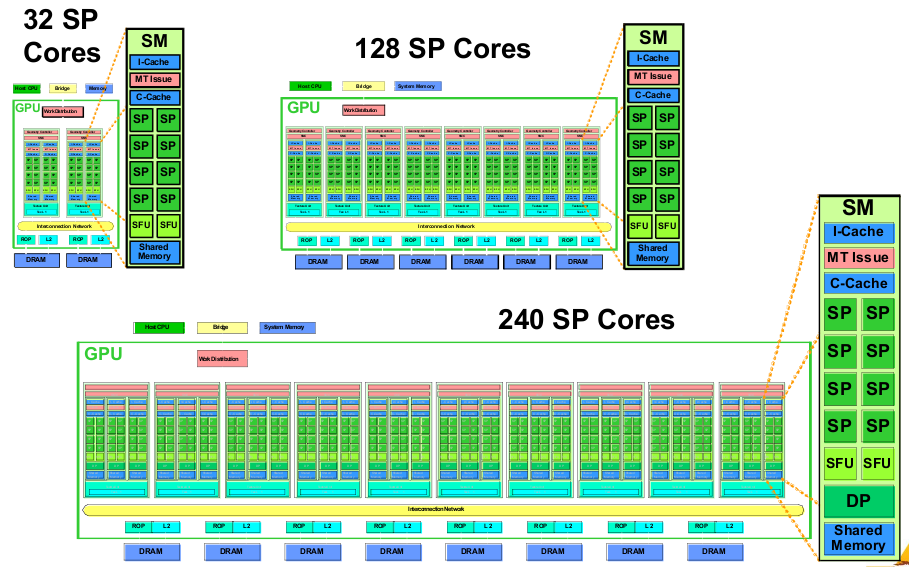
\includegraphics[scale=0.38]{images/1.png}
\end{center}

\end{frame}
%% ============================================================================
%% ============================================================================
\begin{frame}[fragile]
\frametitle{Heterogeneous programming (1/3)}

\begin{itemize}
\item A CUDA program is a serial program with parallel kernels, all in C.
\item The serial C code executes in a \textcolor{blue}{host} (= CPU) thread
\item The parallel kernel C code executes in many \textcolor{blue}{device} 
   threads across multiple GPU processing elements, called 
\textcolor{blue}{streaming processors} (SP).
\end{itemize}

\begin{center}
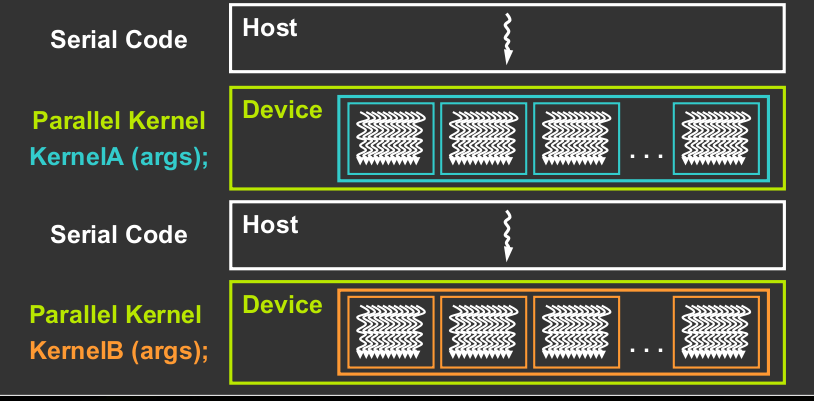
\includegraphics[scale=0.5]{images/Z-17.png}
\end{center}

\end{frame}
%% ============================================================================
%% ============================================================================
\begin{frame}[fragile]
\frametitle{Heterogeneous programming (2/3)}

\begin{itemize}
\item Thus, the parallel code (kernel) is launched and executed on a
      device by many threads.
\item Threads are grouped into thread blocks.
\item One kernel is executed at a time on the device.
\item Many threads execute each kernel.
\end{itemize}

\begin{center}
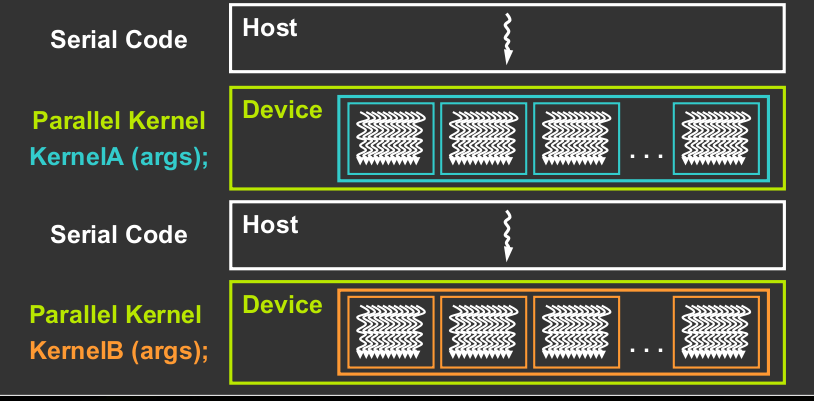
\includegraphics[scale=0.4]{images/Z-17.png}
\end{center}

\end{frame}
%% ============================================================================
%% ============================================================================
\begin{frame}[fragile]
\frametitle{Heterogeneous programming (3/3)}

\begin{itemize}
\item The parallel code is written for a thread
\begin{itemize}
\item Each thread is free to execute a unique code path
\item Built-in \textcolor{blue}{\bf thread and block ID variables}
      are used to map each thread to a specific data tile (see next slide).
\end{itemize}
\item Thus, each thread executes the same code
      on different data based on its thread and block ID.
\end{itemize}

\begin{center}
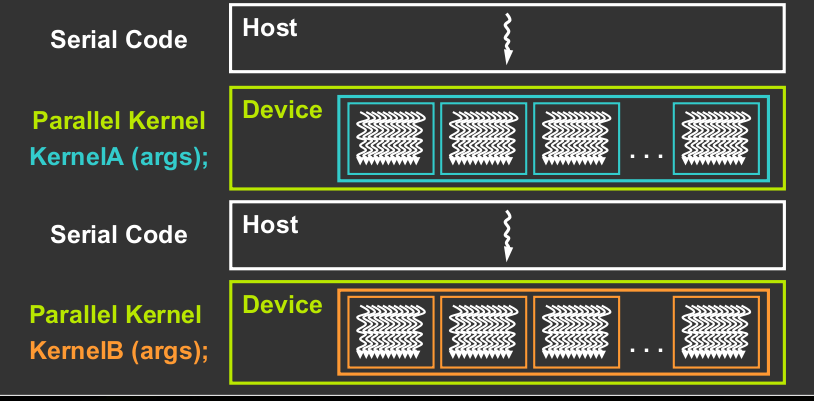
\includegraphics[scale=0.4]{images/Z-17.png}
\end{center}

\end{frame}
%% ============================================================================
%% ============================================================================
\begin{frame}[fragile]
\frametitle{Example: increment array elements (1/2)}

\begin{center}
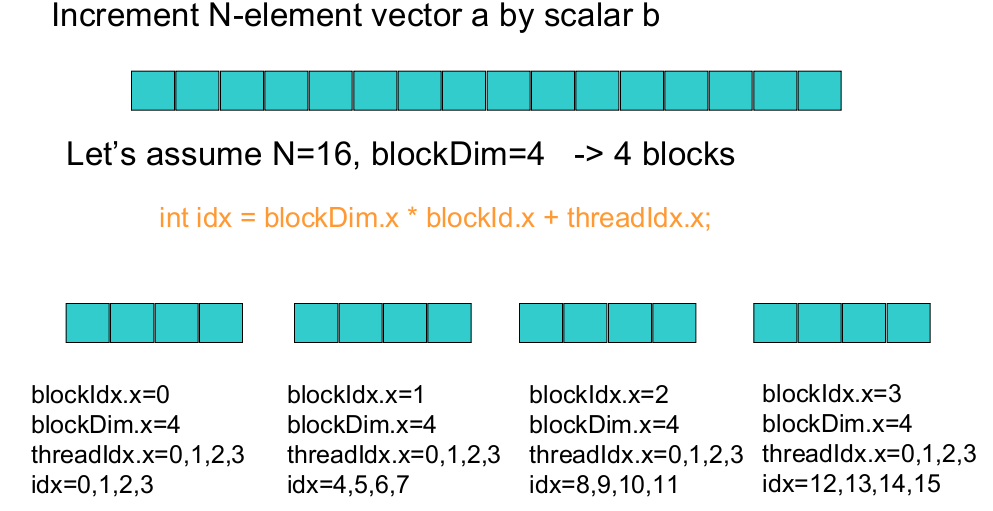
\includegraphics[scale=0.5]{images/7.png}
\end{center}

See our exampe number 4 in {\tt /usr/local/cs4402/examples/4}

\end{frame}
%% ============================================================================
%% ============================================================================
\begin{frame}[fragile]
\frametitle{Example: increment array elements (2/2)}

\begin{center}
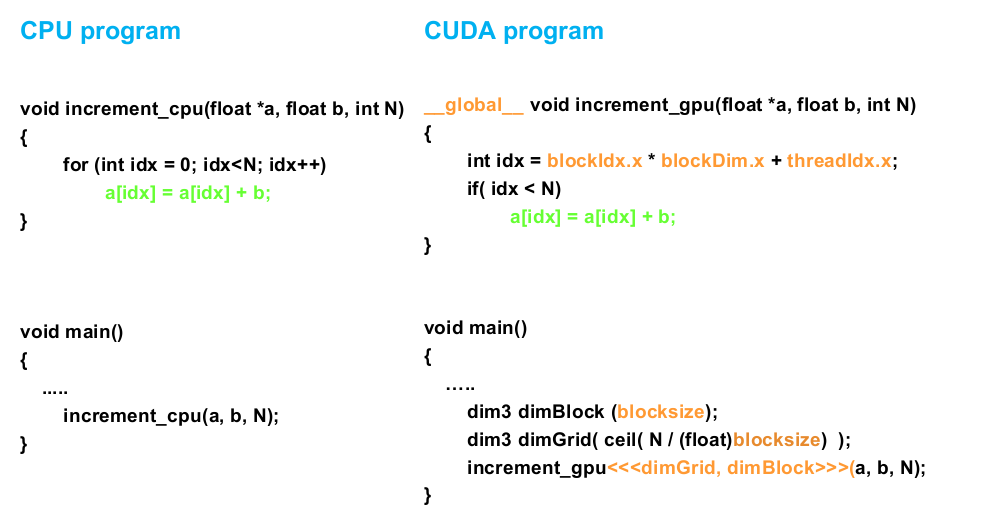
\includegraphics[scale=0.5]{images/8.png}
\end{center}
\end{frame}
%% ============================================================================
%% ============================================================================
\begin{frame}[fragile]
\frametitle{Thread blocks (1/2)}

\begin{itemize}
\item A \textcolor{blue}{\bf Thread block} is a group of threads that can:
\begin{itemize}
\item Synchronize their execution
\item Communicate via shared memory
\end{itemize}
\item Within a grid, \textcolor{red}{\bf thread blocks can run in any order}:
\begin{itemize}
\item  Concurrently or sequentially
\item  Facilitates scaling of the same code across many devices
\end{itemize}
\end{itemize}

\begin{center}
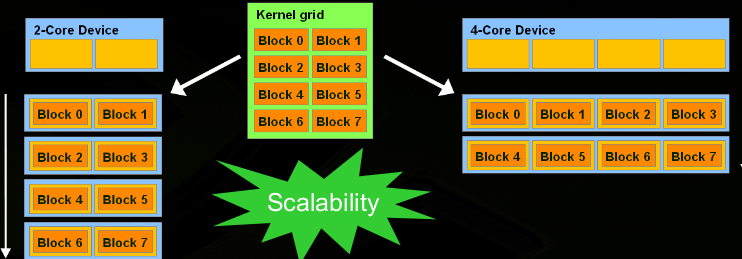
\includegraphics[scale=0.5]{images/11.png}
\end{center}
\end{frame}
%% ============================================================================
%% ============================================================================
\begin{frame}[fragile]
\frametitle{Thread blocks (2/2)}

\begin{itemize}
\item Thus, within a grid, any possible interleaving of 
       blocks must be valid.
\medskip
\item Thread blocks  \textcolor{red}{\bf may coordinate but not synchronize}
\begin{itemize}
\item they may share pointers
\item they should not share locks (this can easily deadlock).
\end{itemize}
\medskip
\item The fact that thread blocks cannot synchronize
     gives \textcolor{blue}{\bf scalability}:
\begin{itemize}
\item A kernel scales across any number of parallel cores
\end{itemize}
\medskip
\item However, within a thread bloc,  
    threads in the same block may synchronize with barriers.
\item That is, threads wait at the barrier until threads 
     in the  \textcolor{red}{\bf same block} reach the barrier.
\end{itemize}

\end{frame}
%% ============================================================================
%% ============================================================================
\begin{frame}[fragile]
\frametitle{Memory hierarchy (1/3)}

\textcolor{blue}{\bf Host (CPU) memory}:
\begin{itemize}
\item Not directly accessible by CUDA threads
\end{itemize}

\begin{center}
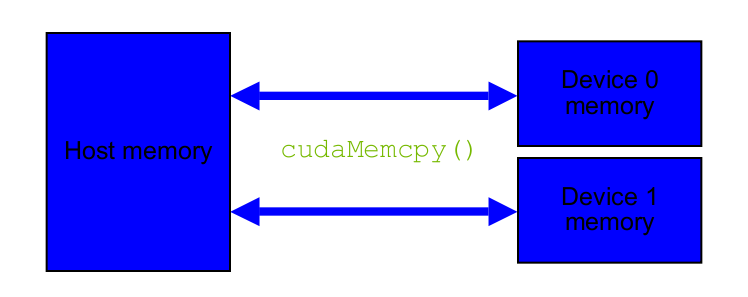
\includegraphics[scale=0.6]{images/15.png}
\end{center}
\end{frame}
%% ============================================================================
%% ============================================================================
\begin{frame}[fragile]
\frametitle{Memory hierarchy (2/3)}

\textcolor{blue}{\bf Global (on the device) memory}:
\begin{itemize}
\item Also called \textcolor{blue}{\bf device memory}
\item Accessible by all threads as well as host (CPU)
\item Data lifetime = from allocation to deallocation
\end{itemize}


\begin{center}
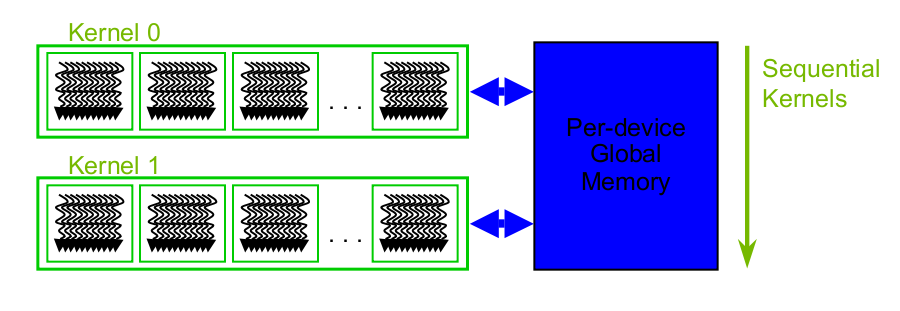
\includegraphics[scale=0.5]{images/14.png}
\end{center}
\end{frame}
%% ============================================================================
%% ============================================================================
\begin{frame}[fragile]
\frametitle{Memory hierarchy (3/3)}

\textcolor{blue}{\bf Shared memory}:
\begin{itemize}
\item  Each thread block has its own shared memory,
       which is accessible only by the threads within that block
\item Data lifetime = block lifetime
\end{itemize}

\textcolor{blue}{\bf Local storage}:
\begin{itemize}
\item Each thread has its own local storage
\item Data lifetime = thread lifetime
\end{itemize}

\begin{center}
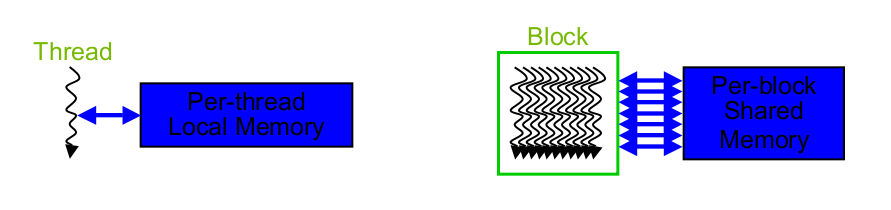
\includegraphics[scale=0.5]{images/13.png}
\end{center}
\end{frame}
%% ============================================================================
%% ============================================================================
\begin{frame}[fragile]
\frametitle{Blocks run on multiprocessors}


\begin{center}
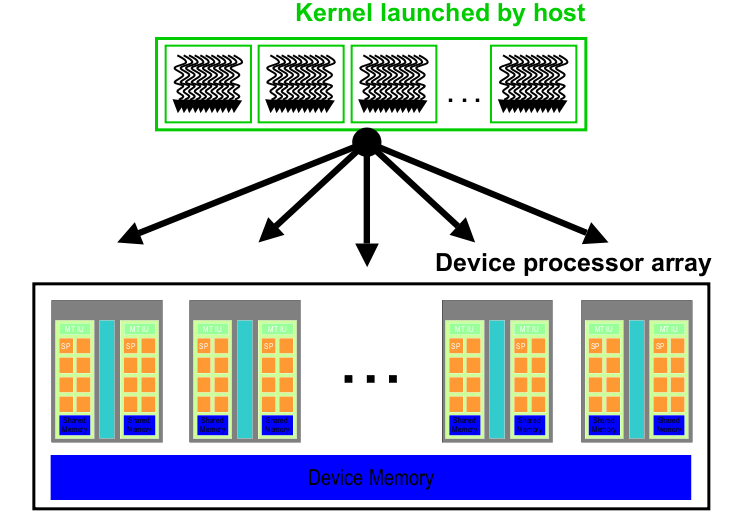
\includegraphics[scale=0.5]{images/41.png}
\end{center}
\end{frame}
%% ============================================================================
%% ============================================================================
\begin{frame}[fragile]
\frametitle{Streaming processors and multiprocessors}

\begin{center}
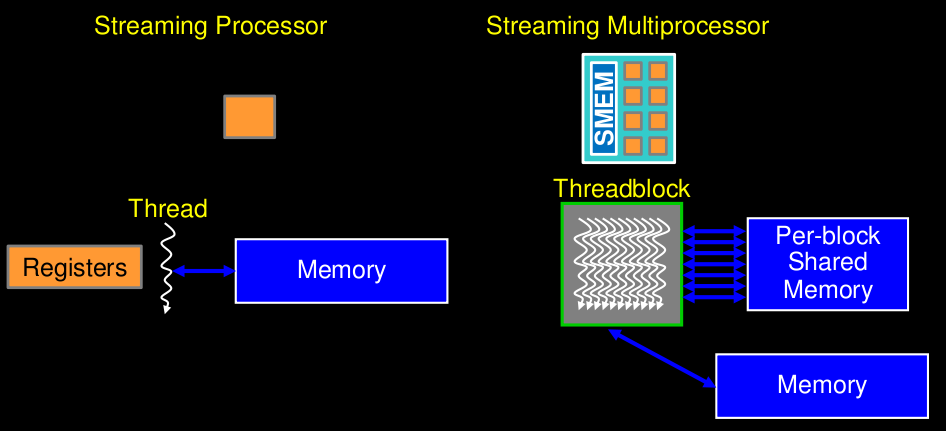
\includegraphics[scale=0.5]{images/S-6.png}
\end{center}
\end{frame}
%% ============================================================================
%% ============================================================================
\begin{frame}[fragile]
\frametitle{Hardware multithreading}

\begin{itemize}
\item \textcolor{blue}{\bf Hardware allocates resources to blocks}:
\begin{itemize}
\item blocks need: thread slots, registers, shared memory
\item blocks don't run until resources are available
\end{itemize}
\item \textcolor{blue}{\bf Hardware schedules threads}:
\begin{itemize}
\item hreads have their own registers
\item any thread not waiting for something can run
\item context switching is free – every cycle
\end{itemize}
\item \textcolor{blue}{\bf Hardware relies on threads to hide latency}:
\begin{itemize}
\item thus high  parallelism is necessary for performance.
\end{itemize}
\end{itemize}


\begin{center}
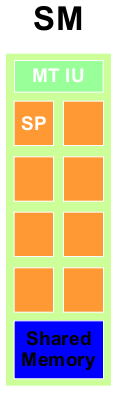
\includegraphics[scale=0.35]{images/39.png}
\end{center}
\end{frame}
%% ============================================================================
%% ============================================================================
\begin{frame}[fragile]
\frametitle{SIMT thread execution}

\begin{itemize}
\item  At each clock cycle, a   
      multiprocessor executes the same
     instruction on a group of threads
     called a \textcolor{blue}{\bf warp}
\begin{itemize}
\item  The number of threads in a warp is
      the \textcolor{blue}{\bf warp size} (32 on G80)
\item A half-warp is the first or second
      half of a warp.
\end{itemize}
%%
\item  Within a warp, threads
\begin{itemize}
%% \item always executing same instruction
\item  share instruction fetch/dispatch
\item  some become inactive when code path diverges
\item  hardware automatically handles divergence
\end{itemize}
%%
\item   \textcolor{blue}{\bf  Warps are the primitive unit of scheduling}:
\begin{itemize}
\item each active block is split nto warps in a well-defined way
\item threads within a warp are executed physically in
      parallel while warps and blocks are executed logically in
      parallel.
\end{itemize}
\end{itemize}

\begin{center}
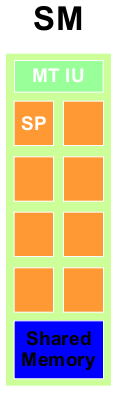
\includegraphics[scale=0.25]{images/39.png}
\end{center}
\end{frame}
%% ============================================================================


%%%%%%%%%%%%%%%%%%%%%%%%%%%%%%%%%%%%%%
\section{Fast Polynomial Arithmetic} %
%%%%%%%%%%%%%%%%%%%%%%%%%%%%%%%%%%%%%%

\begin{frame}
%%\frametitle{Background: fast polynomial arithmetic over finite fields}
\frametitle{Background}
\begin{block}{Goal}
Accelerate dense polynomial arithmetic using GPUs   
\end{block}
\begin{block}{Polynomial multiplication over finite fields}
%%The building block of symbolic computation
\begin{itemize}
\item many algorithms rely on polynomial multiplications
\item \textcolor{red}{modular methods} reduce the computations to finite fields
\item fast algorithms like FFT exist
\end{itemize}
\end{block}
\begin{block}{Fast Fourier Transform (FFT) over finite fields}
$$f \times g = \FFT^{-1} (\FFT(f) \cdot \FFT(g))$$
Challenges comparing to $\FFT$s over \textcolor{red}{complex numbers}:
\begin{itemize}
\item radix 2 $\FFT$ is desirable, keeping other primes invertible 
\item lack of primitive roots of unity, (when the degree is high)
\item modular multiplication is expensive
\end{itemize}
\end{block}
\end{frame}

%% ============================================================================
%% ============================================================================
\begin{frame}
\frametitle{Discrete Fourier Transform (DFT)}



\begin{block}{Definition}
Given a primitive $n$-th root of unity $\omega$ (i.e. $\omega^{n/2} = -1$), 
and $$f(t) = x_0 + x_1t + \cdots + x_{n-1}t^{n-1},$$
${\mathrm{{DFT}}}_n^{\omega}(f) $ is $\mathbf{y} = (y_0, \ldots, y_{n-1})$ with 
\textcolor{blue}{$y_k = f(\omega^{k})$ for $0 \leq k < n$}. 
As a matrix-vector product, it is
\begin{equation}
\mathbf{y} = {\mathrm{DFT}}_n\, \mathbf{x},\quad 
\mathrm{DFT}_n = [\omega^{k\ell}]_{0\leq k,\, \ell < n}. 
\end{equation}
\end{block}


\begin{block}{Example}
$$\left\{ 
    \begin{array}{ccc} 
        y_0 & = & x_0 + x_1 \\ 
        y_1 & = & x_0 - x_1 
  \end{array}\right.
\Longleftrightarrow
\begin{bmatrix} y_0 \\ y_1 \end{bmatrix} 
= \begin{bmatrix} 1 & 1 \\ 1 & -1
\end{bmatrix}
\begin{bmatrix} x_0 \\ x_1 \end{bmatrix}$$
That is, $\DFT_2 = \left[\begin{array}{cr} 1 & 1\\ 1 & -1 \end{array}\right]$.
\end{block}

\end{frame}
%% ============================================================================

%% ============================================================================
\begin{frame}
\frametitle{FFT-based multiplication}

\textcolor{darkred}{M(d)}  number of coefficient operations in degree less than  \textcolor{darkred}{d}.

\begin{tabular}[t]{|l|l|}
\hline
Classical Multiplication & \textcolor{darkred}{$\M(d)~=~2d^2$}\\
\hline
Karatsuba Multiplication & \textcolor{darkred}{$\M(d)~=~9d^{1.59}$} \\
\hline
FFT over appropriate ring & \textcolor{darkred}{$\M(d)~=~9/2 d\,\log d + 3 \, d$} \\  \hline
\end{tabular}

\bigskip 

\fbox{
\begin{minipage}{10 cm}
\begin{description}
\item[{\bf Input:}] $f, g \in {\K}[x]$ and ${\omega}$ a $s$-primitive
                    root of unity for $s > {\deg}(f) + {\deg}(g)$
                    and $s$ is a power of $2$.
\item[{\bf Output:}] the product $fg$
\end{description}
\begin{tabbing} 
\quad \= \quad \= \quad \= \quad \kill
(1) \> \> Evaluate $f$ and $g$ at ${\omega}^i$ for $i = 0 \cdots s-1$ \\
(2) \> \> Evaluate $fg$ at ${\omega}^i$ for $i = 0 \cdots s-1$ \\
(3) \> \> Interpolate and {\bf return} $fg$
\end{tabbing}
\end{minipage}
}
See (M.M.M. Yuzhen Xie 2009) for implementation techniques.

\end{frame}
%% ============================================================================

%% ============================================================================
\begin{frame}
\frametitle{The fast division trick (1/2)}


\begin{itemize}
\item Let $a, b \in {\A}[x]$ with $n := {\deg}(a) \geq m := {\deg}(b) > 0$,
\red{$b$ monic} and {\A} any commutative ring with 1.
\medskip
\item<2-> We want the \blue{\sf  quotient} $q$ 
and the \blue{\sf  remainder} $r$ of $a$ w.r.t. $b$:
\begin{center}
$a(x) \ = \ q(x) \, b(x) + r(x)$
\end{center}
\medskip
\item<3-> Replacing $x$ by $1/x$ and multiplying the equation by $x^n$:
$$x^n \, a(1/x) \ = \ \left(x^{n-m} q(1/x) \right) \ 
                    \left(x^m \, b(1/x) \right) \ + \ x^{n-m+1} \left( x^{m-1} \,  r(1/x) \right) $$
That is:
\begin{center}
\red{$ {\rm rev}_n (a) \ = \ {\rm rev}_{n-m}(q) \ {\rm rev}_m (b) +  x^{n-m+1} \ {\rm rev}_{m-1}(r) $}
\end{center}
\medskip
\item<4-> Computing 
\red{$( {\rm rev}_m (b))^{-1} \mod{  x^{n-m+1}}$} 
is a \blue{\sf truncated inverse of a power series}.
(S. Cook, 1966) (H. T.  Kung, 1974) and (M. Sieveking, 1972)
\end{itemize}

\end{frame}
%% ============================================================================
\ifshow
\fi

%% ============================================================================
\begin{frame}
\frametitle{The fast division trick (2/2)}

\fbox{
\begin{minipage}{10 cm}
\begin{description}
\item[{\bf Input:}] $f \in {\A}[x]$ such that $f(0) = 1$ and ${\ell} \in {\N}$.
\item[{\bf Output:}] $g \in {\A}[x]$ such that $f \, g \equiv 1 \mod{ \ x^{\ell}}$
\end{description}
\begin{tabbing} 
\quad \= \quad \= \quad \= \quad \kill
\> $g_0$ := $1$ \\
\> $r$ := $\lceil {\log}_2({\ell}) \rceil$ \\
\> {\bf for} $i = 1 \cdots r$ {\bf repeat} \\
\> \> $g_i$ := $\left( 2 g_{i-1} - f \, {g_{i-1}}^2 \right) \ \mod{ \ x^{2^i}} $ \\
\> {\bf return} $g_r$
\end{tabbing}
\end{minipage}
}

\medskip

\begin{itemize}
\item  This algorithm runs in $3 {\M}(\ell) + 0(\ell)$ 
operations in ${\A}$. 
\item Improved versions run in $2\,{\M}(\ell) + O({\ell})$ 
operations in ${\A}$. 
\item Finally, the \blue{\sf  quotient} $q$ 
and the \blue{\sf remainder} $r$ are computed 
in $3 \, {\M}(n - m) + {\M}({\max}(n-m,m)) + {\cal O}(n)$
operations in ${\A}$
\item {\em Modern Computed Algebra} (Gathen Gerhard 99)
\end{itemize}

\end{frame}


%%%%%%%%%%%%%%%%%%%%%%%%%%%%%%%%%%%%%%
\section{Subproduct Tree Techniques} %
%%%%%%%%%%%%%%%%%%%%%%%%%%%%%%%%%%%%%%
%% ============================================================================
%% ============================================================================
\begin{frame}[plain]{Subproduct trees}
\fontsize{8}{9}\selectfont  
{
\begin{itemize}
	\item Useful construction to devise \textcolor{blue}{fast algorithms} with univariate polynomials,
	\item If $m_0, m_1,\ldots , m_{n-1}$ are monic, non-constant, polynomials in ${\K}[x]$, then their subproduct tree can be constructed in $O(M(d)\log_2(n))$ operations in {\K}
where  $d = \sum_{i=0}^{n-1}\degree{m_i}$.
\end{itemize}
}	
\begin{figure}[htb] %htb
  \begin{center}
  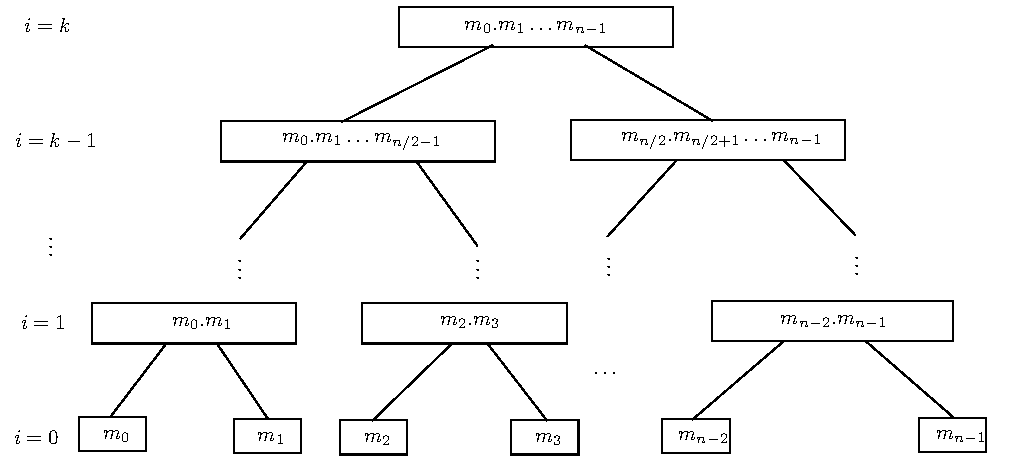
\includegraphics[scale=0.6]{images/sptree2.pdf} %width=6.4in,height=3.0in
  \end{center}
\end{figure}	
\end{frame} 
%% ============================================================================
%% ============================================================================
\begin{frame}[plain]{Fast multiple remainders}

\fontsize{8}{9}\selectfont  
{
\begin{itemize}
\item Let $m_0, m_2,\ldots , m_{n-1}$ be as before and assume their subproduct tree $M$
      has been computed. Let $f \in {\K}[x]$ be a polynomial of degree less than $d$.
\item To compute $f  \ {\rm rem} \ m_0, f  \ {\rm rem} \ m_1,\ldots , f  \ {\rm rem} \ m_{n-1}$, 
      one reduces $f$ by the root of $M$, then by its children (leading to two remainders)
      and so on.
\item This amounts to $O(M(d)\log_2(n))$ operations in {\K}.
\end{itemize}
}

\begin{figure}[htb] %htb
  \begin{center}
  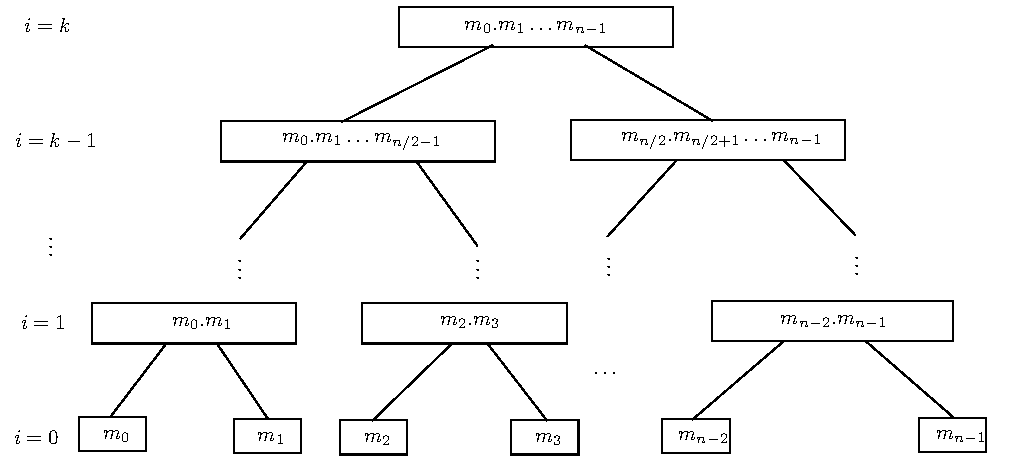
\includegraphics[scale=0.5]{images/sptree2.pdf} %width=6.4in,height=3.0in
  \end{center}
\end{figure}

\end{frame} 
%% ============================================================================
%% ============================================================================
\begin{frame}[plain]{Fast evaluation}

\fontsize{8}{9}\selectfont  
{
\begin{itemize}
\item Suppose the polynomials $m_0, m_2,\ldots , m_{n-1}$ are of the form
      $x - x_0, x- x_1, \ldots, x - x_{n-1}$, where
      $x_0, x_1, \ldots, x_{n-1}$ are pairwise values in {\K}.
\item In this case, the procedure for fast multiple remainders
      provides a procedure for \blue{mulit-point evaluation}
      running in $O(M(d)\log_2(d))$ operations in {\K}.
\item This is a significant improvement w.r.t Horner's Rule
      which runs in $O(d^2)$ operations in {\K}.
\end{itemize}
}

\begin{figure}[htb] %htb
  \begin{center}
  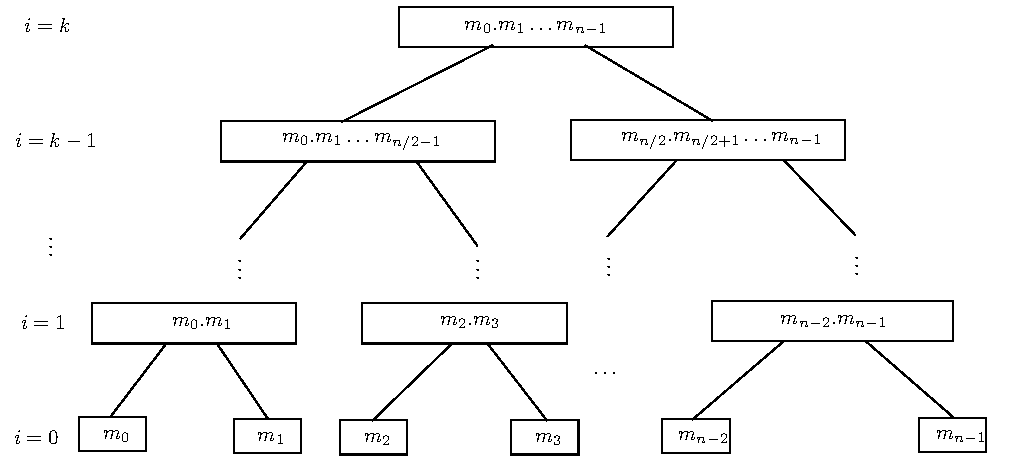
\includegraphics[scale=0.5]{images/sptree2.pdf} %width=6.4in,height=3.0in
  \end{center}
\end{figure}

\end{frame} 


%%%%%%%%%%%%%%%%%%%%%%%%%%%%%%%%%%%%%%
\section{Implementation in CUDA}     %
%%%%%%%%%%%%%%%%%%%%%%%%%%%%%%%%%%%%%%
%% ============================================================================
%% ============================================================================
\begin{frame}
\frametitle{Subproduct tree representation in CUDA}

\begin{itemize}
\item A subproduct tree on $n = 2^k$ points consists
      of $k$ levels (not counting the root).  
\item At level $h = 0$ (the leaves)
      we have $2^k$ polynomials of degree $2^0$, amounting to 
       $2^k (2^0 + 1)$ coefficients in total.
\item At level $h$, we have $2^{k-h}$ polynomials of degree $2^h$, amounting to 
       $2^{k-h} (2^h + 1)$ coefficients in total.
\item The total number of coefficients is
\begin{equation*}
2^{k+1} + k 2^k -2
\end{equation*}
\item Assuming that each coefficient requires 4 bytes and that
our GPU has 3 Giga-bytes of global memory, the largest possible $k$ is $24$.
\item In the GPU global memory, the subproduct tree is an array
      storing successively the polynomials at lelvel $h=0$, $h=1$,
     \ldots $h = k -1$.
\end{itemize}
\end{frame}
%% ============================================================================
%% ============================================================================
\begin{frame}
\frametitle{Polynomial multiplication in CUDA}
\begin{itemize}
\item We rely on FFT-based multiplication in input degree higher than $2^8$.
      (M.M.M. \& Wei Pan, Journal of Physics Conference Series, 2011).
\item In lower degree, we rely in plain quadratic multiplication.
\item The table below compares our FFT-based multiplication and an
      optimized plain multiplication for 
       $(t, w) \in \{ (128, 4), (128, 8),  (256, 4), (256, 8) \}$
      where $t$ is the numberof threads per block and $w$
       the number of coefficients per thread.
\end{itemize}

\begin{tabular}{ l || l | l | l | l | l |l |}
\hline
Length & FFT-based & Opt 1 & Opt 2 & Opt3 & Opt4 \\
\hline
8 & 4.168448 & 0.147488 & 0.138048 & 0.151136 & 0.140608 \\
9 & 3.866848 & 0.230976 & 0.157984 & 0.215872 & 0.159136 \\
10 & 5.014496 & 0.513888 & 0.334464 & 0.496096 & 0.305600 \\
11 & 5.299264 & 1.667808 & 0.870688 & 1.875936 & 0.964352 \\
12 & 5.944992 & 6.31552 & 3.115360 & 7.439104 & 3.572864 \\
13 & 6.267520 & 25.045984 & 12.077248 & 29.626495 & 14.270720\\
14 & 7.050112 & 20.753984 & 47.733665 & 64.931938 & 57.355328\\
\hline
\end{tabular}

\end{frame}

%% ============================================================================
%% ============================================================================
\begin{frame}
\frametitle{Subproduct tree construction in CUDA (1/3)}

\begin{itemize}
\item The subproduct tree is built bottom-up, starting from the leaves.
\item Building level $h+1$ from level $h$ is done by a series of CUDA kernel calls.
\item Each level from $h=0$ to $h=7$ involves multiplication in degree $2^7$ or less,
      thus it is performed by a \blue{list of plain multiplications}.
\item Each of the higher levels requires FFT-based multiplication, thus
        \blue{list of direct FFTs}, followed by 
         \blue{list of pointwise multiplications}, followed by 
      \blue{list of inverse FFTs}.
\end{itemize}
\end{frame}
%% ============================================================================
%% ============================================================================
\begin{frame}[shrink=20]
\frametitle{Subproduct tree construction in CUDA (2/3)}
\begin{tabular}{l || l | l}
Input Size (${\log}_2$ of) & Time (ms) & Memory (Bytes)\\
\hline
%% 3 & 0.057280 & 56\\
4 & 0.070720 & 152\\
5 & 0.111808 & 376\\
6 & 0.323840 & 888\\
7 & 0.468992 & 2040\\
8 & 0.829888 & 4600\\
9 & 1.995616 & 10232\\
10 & 5.477760 & 22520\\
11 & 8.468224 & 49144\\
12 & 12.787584 & 106488\\
13 & 15.839264 & 229368\\
14 & 24.897984 & 491512\\
15 & 35.802338 & 1048568\\
16 & 56.436737 & 2228216\\
17 & 89.414787 & 4718584\\
18 & 161.420929 & 9961464\\
19 & 298.262054 & 20971512\\
20 & 587.439819 & 44040184\\
21 & 1180.089966 & 92274680\\
22 & 2308.174072 & 192937976\\
23 & 4549.854980 & 402653176\\
24 & 8180.691895 & 838860792\\
\end{tabular}
\end{frame}
%% ============================================================================
%% ============================================================================
\begin{frame}
\frametitle{Subproduct tree construction in CUDA (3/3)}
\begin{center}
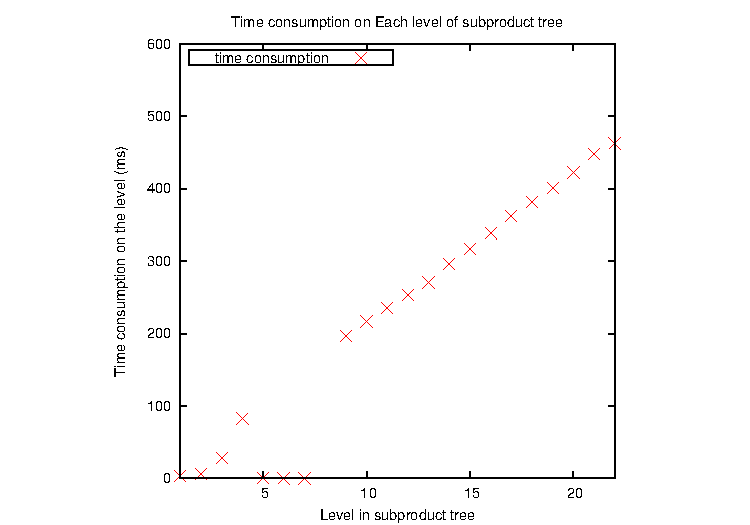
\includegraphics[scale=0.9]{images/sub_product_tree_step.pdf}
\end{center}
\end{frame}
%% ============================================================================
%% ============================================================================
\begin{frame}
\frametitle{Fast multi-point evaluation in CUDA (1/3)}
\begin{itemize}
\item The fast multi-point evaluation proceeds in a top-down manner.
\item Moving from lelvel $h$ down to level $h-1$ is done by a series of CUDA kernel calls.
\item Each level from $h=0$ to $h=7$ involves plain division.
\item Each of the higher levels uses \blue{fast division}.
\item The \blue{power series inversion} uses plain (quadratic) multiplications in low
      degree and FFT-based multiplication from degree $2^8$.
\end{itemize}
\end{frame}
%% ============================================================================
%% ============================================================================
\begin{frame}[shrink=20]
\frametitle{Fast multi-point evaluation in CUDA (2/3)}
\begin{tabular}{ l | l }
Input size  (${\log}_2$ of)  & Time (ms) \\
\hline
% 2 & 0.066016 \\
% 3 & 0.039424 \\
4 & 0.064032 \\
5 & 0.102784 \\
6 & 0.176448 \\
7 & 0.320640 \\
8 & 0.627616 \\
9 & 1.181408 \\
10 & 2.019488 \\
11 & 53.894718 \\
12 & 113.643204 \\
13 & 178.820190 \\
14 & 261.687347 \\
15 & 360.460541 \\
16 & 511.921570 \\
17 & 791.367065 \\
18 & 1216.930176 \\
19 & 2084.443359 \\
20 & 3773.393066 \\
21 & 7177.844238 \\
22 & 14181.632812 \\
23 & 28927.501953 \\
\end{tabular}
\end{frame}
%% ============================================================================
%% ============================================================================
\begin{frame}
\frametitle{Fast multi-point evaluation in CUDA (3/3)}
\begin{center}
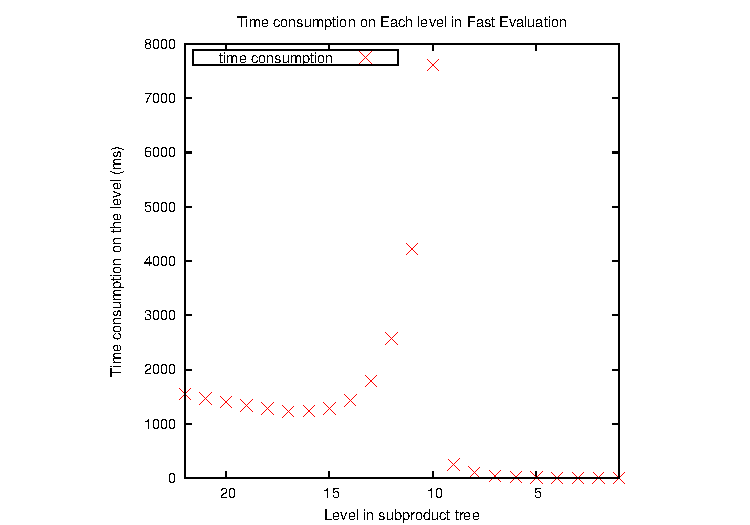
\includegraphics[scale=0.9]{images/fast_evaluation_step.pdf}
\end{center}
\end{frame}
%% ============================================================================
%% ============================================================================
\begin{frame}
\frametitle{Conclusions}

\end{frame}
%% ============================================================================


\end{document}



\begin{frame}
%%%%%%%%%%%%%%%%%%%%%%%%%%%%%%%%
\frametitle{Summary and notes} %
%%%%%%%%%%%%%%%%%%%%%%%%%%%%%%%%


\end{frame}

